\documentclass[twocolumn]{article}
\usepackage{amsmath}
\usepackage{amssymb}
\usepackage{enumitem}
\usepackage[most]{tcolorbox}
\usepackage{xcolor}
\usepackage{natbib}
\usepackage{siunitx}
\usepackage{tikz}
\usepackage{textcomp} % Useful for symbols like \textdegree
\usepackage{hyperref}
% Define a new tcolorbox environment for literature papers
\newtcolorbox{literaturepaper}[1]{ % #1 is for the title
    enhanced,
    breakable, % Allows the box to break across pages/columns
    colback=gray!5,
    colframe=black!20,
    boxsep=5pt,
    arc=4pt,
    title={#1}, % Title is the mandatory argument
    fonttitle=\bfseries,
    coltitle=blue!70!black,
    span=all, % Makes the box span all columns
    parbox=false, % Allows paragraphs to break correctly within the box
    before skip=1em,
    after skip=1em,
    left skip=0pt,
    right skip=0pt
    % 'growboxset' was removed as it's not a standard tcolorbox key;
    % height is usually managed automatically by 'breakable' and content.
}

% A new tcolorbox for small highlighted blocks (display style)
\newtcolorbox{smallhighlightbox}[1][]{
    enhanced,
    colback=blue!5!white,
    colframe=blue!20!white,
    boxsep=2pt,
    arc=2pt,
    boxrule=0.5pt,
    #1
}

\bibliographystyle{plainnat} % Or another style like abbrvnat, unsrtnat

\begin{document}

\section*{Literature Summaries}
\vspace{0em}
    \large\textit{Summaries compiled by \textbf{Bryan L.A.}, Amsterdam, NL. 2025.}
\vspace{1em}

% First literature summary box
\begin{literaturepaper}{Bayesian Graphical Models for Integrating Multiplatform Genomics Data \cite{Wang_Baladandayuthapani_Holmes_Do_2013}}
\label{paper-summary-1}
\small
    \textbf{Aim:} Graphical model frameworks to integrate multiplatform genomic data (gene expression and microRNA expression) with clinical data (patient survival) to identify and characterize meaningful biological relationships. Model selection problem: For each triplet, select best-fitting graph from $K_i$ (determine type of dependence structure). Focus on identifying mRNA and genes whose relationship align with biologically plausible processes.

    \textbf{G} = Gene expression, \textbf{M} = MicroRNA expression, \textbf{C} = Clinical outcome
    
    \begin{itemize}[label=$\circ$]
        \item Undirected graphs where each node is either $G, M, C$.
        \item Let $V = \{G,M,C\}$ be set of nodes (variables) in graphs.
        \item Each of the 8 models represented as undirected graphs $K_i$ (for $i = 0,...,7$).
        \item $K_i = (V, E_i)$, where an edge $(u, v) \in E_i$ signifies Conditional Dependence (direct statistical association) between $u$ and $v$.
        \item Absence of $(u, v)$ means nodes are conditionally independent given a 3rd variable.
    \end{itemize}

    \textbf{Statistical framework:} Bayesian model selection approach for Gaussian graphical models (GGMs) to select most appropriate $K_i$ for each $V$. Bayesian GGM has closed-form expression $\to$ reduced computational time/cost.

    Whereas molecular features at DNA level only modulate mRNA expression of corresponding (nearby) genes, microRNA can regulate mRNA expression of any genes regardless of locus (also multiple target capability). Relationship between microRNA and targets depends ONLY on inherent features (such as sequence and structure of microRNA).

    \textbf{GGM:} For measuring dependency structure for multivariate normal distributions.

    Let $X = (x_1,...,x_p)'$ be a $p$-dimensional normal random vector with mean $\mu$ and covariance matrix $\Sigma$.
    Each observation $x \sim N(0, \Sigma)$, with unknown $\Sigma$.
    
    \textbf{\textit{Inverse covariance matrix}} (Precision matrix/Concentration matrix) $\Omega = \Sigma^{-1}$ reveals \textbf{\textit{conditional dependence structure}}. $\Omega$ has elements $\omega_{ij}$.
    An off-diagonal element $\omega_{ij} = 0$ (for $i \neq j$) if and only if variables $x_i$ and $x_j$ are \textbf{conditionally independent} given all other variables in the set.
    Partial correlation: $\rho_{ij \cdot \text{rest}} = -\omega_{ij} / \sqrt{\omega_{ii}\omega_{jj}}$.

    When \textbf{off-diagonal elements} $\omega_{ij} = 0$ (for $i \neq j$), this implies NO EDGE, meaning no direct relationship (after accounting for the influence of all other variables $X_{V \setminus \{i,j\}}$).

    Partial correlation thus measures \textit{direct linear association} between 2 variables AFTER adjusting/removing for linear effects of all other variables in the model, helping to distinguish \textbf{direct} from \textbf{indirect} relationships.

    \textbf{Conditional variance of $x_i$:} is $1/\omega_{ii}$ (assuming $\Omega$ is the precision matrix of the conditional distribution). Increasing $\omega_{ii}$ means decreasing conditional variance (higher precision).

    \textbf{Multivariate Normal Density Function:} $\Omega$ appears in the exponent:
    \[f(X) \propto \exp\left(-\frac{1}{2}(X-\mu)'\Omega(X-\mu)\right)\]
    The term $(X-\mu)'\Omega(X-\mu)$ is a quadratic form defining the \textbf{Mahalanobis distance} (\textit{measures distance between a point and a distribution, accounting for covariance}). Here, $\Omega$ determines the shape of the distribution.

    \textbf{Geometrical meaning:} Surfaces of constant probability density are \textit{ellipsoids} (isoprobability contours). Their shape, orientation, and tightness are determined by $\Sigma$ (and thus $\Omega$).

    $\Omega$ is \textbf{diagonal} $\rightarrow$ all \textbf{off-diagonal elements} $\omega_{ij} = 0$ (for $i \neq j$), while \textbf{diagonal elements} $\omega_{ii}$ can be non-zero.

    \textbf{Decomposable Graph:} $G = (V,E)$ if either G is complete or $V = A \cup S \cup B$, where $S$ is \textbf{complete} and separates $A$ and $B$, and both $A \cup S$ and $B \cup S$ are decomposable graphs. (All 8 models in the chapter are stated to be decomposable).

    Posterior probability of graph $G$:
    \[p(G|X) \propto p(G) \int p(X|\Sigma, G) p(\Sigma|G) d\Sigma,\]
    where $p(G)$ is the prior for graph $G$, and $p(\Sigma|G)$ is the prior for covariance matrix $\Sigma$ given $G$.

    \textbf{Prior Choice:} The integral is sensitive to the choice of prior $p(\Sigma|G)$.
    \textbf{Hyper-inverse Wishart (HIW) distribution:} A conjugate prior, $p(\Sigma|G) \sim \text{HIW}_G(b, D)$, where $b$ is for degrees of freedom and $D$ is a scale matrix.
    
    \textbf{Fractional Bayes Factors:} Used when prior information is weak. Notionally uses a small fraction $(g)$ of the data (likelihood) to "train" a noninformative prior into a proper one.
    The HIW g-prior, $p(\Sigma|G) \sim \text{HIW}_G(g \cdot n, gX'X)$, corresponds to this fractional Bayes factor approach, addressing the "double use of data" concern from $X'X$ in the prior.

    \textbf{Bayes Factor $BF(G_0 : G_i)$ for comparing null graph $G_0$ (no edges) to an alternative $G_i$:}
    (\textit{Your transcribed formula. Note: The product terms over cliques $\mathcal{C}$ and separators $\mathcal{S}$ in your transcription of $F_i$ are identical in the numerator and denominator and would cancel out. Please verify if this is the intended formula. The formula in `4.pdf` (Equation 14.2) is different.})

    Let the Bayes Factor be $BF(G_0 : G_i) = M \times F_i$, where $F_i$ is the main fraction:
    \[ F_i = \frac{\prod_{j=1}^p \left|\frac{1}{2}X_j'X_j\right|^{\frac{n}{2}} \prod_{C \in \mathcal{C}} \left|\frac{1}{2}X_C'X_C\right|^{\frac{|C|}{2}}\prod_{S \in \mathcal{S}} \left|\frac{1}{2}X_S'X_S\right|^{\frac{|S|}{2}}}{\prod_{j=1}^p \left|\frac{1}{2n}X_j'X_j\right|^{\frac{1}{2}} \prod_{S \in \mathcal{S}} \left|\frac{1}{2}X_S'X_S\right|^{\frac{|S|}{2}} \prod_{C \in \mathcal{C}} \left|\frac{1}{2}X_C'X_C\right|^{\frac{|C|}{2}}} \]
    And $M$ is:
    \[ M = \frac{\prod_{C \in \mathcal{C}} \Gamma\left(\frac{n+|C|-1}{2}\right) \prod_{S \in \mathcal{S}} \Gamma\left(\frac{|S|}{2}\right)}{\prod_{S \in \mathcal{S}} \Gamma\left(\frac{n+|S|-1}{2}\right)\prod_{C \in \mathcal{C}} \Gamma\left(\frac{|C|}{2}\right)} \]

    \textbf{Example of $\Omega$ matrices:}
    General $\Omega$:
    \[ \Omega = \begin{pmatrix} \omega_{11} & \omega_{12} & \omega_{13} \\ \omega_{21} & \omega_{22} & \omega_{23} \\ \omega_{31} & \omega_{32} & \omega_{33} \end{pmatrix} \]
    Diagonal $\Omega$:
    \[ \Omega_{\text{diagonal}} = \begin{pmatrix} \omega_{11} & 0 & 0 \\ 0 & \omega_{22} & 0 \\ 0 & 0 & \omega_{33} \end{pmatrix} \]

    \textbf{Preprocessing step for clinical outcome C (in GGM context):} Use Cox model and Breslow estimator to handle censored survival data and derive a transformed (e.g., imputed, log-transformed) clinical outcome variable 'C' suitable for the GGM framework.
\end{literaturepaper} % Correct placement for the end of the first paper's box

% Second literature summary box
\begin{literaturepaper}{SVNN: an efficient PacBio-specific pipeline for structural variations calling using neural networks \cite{Akbarinejad2021}}
\label{paper-summary-2}
\small
    \textbf{Aim:} Structural Variations (SV) - insertion/deletion/translocation/inversion $> 50\text{bp}$ - significant contributors to human disease and phenotypic traits. While long sequencing reads are better for detecting large SVs, they suffer from high sequencing error rates (up to $15\%$). Therefore, high-coverage data is needed for accurate SV detection, making the alignment phase (prerequisite for SV calling) extremely time-consuming and costly. Long-read SV analyses often deal with low-coverage data. There is a need for an efficient SV calling pipeline.

    \textbf{Proposed solution:} SVNN, a fast and accurate PacBio-specific pipeline for calling SVs $> 50\text{bp}$ from raw long-reads. Aims for high sensitivity and precision even in low-coverage settings while being faster than naive combinations of state-of-the-art tools.

    \textit{SVNN combines existing tools using a Neural Network (NN) to optimize speed and accuracy. It leverages fast aligners for initial processing and more accurate (albeit slower) aligners only for a crucial subset of reads identified by the NN.}

    \textbf{Stages/Modules}
    \begin{itemize}
        \item \textbf{Map with Minimap2:} All raw input reads are mapped to reference genome using Minimap2 (fast long-read aligner).
        \item \textbf{Find Informative Reads (NN):}
        \begin{itemize}
            \item Features are extracted from the SAM file output (from module 1) for each read.
            \item Pre-trained NN classifies reads into 2 categories:
            \begin{itemize}
                \item \textbf{Informative reads:} Reads not split by Minimap2 but likely to be split by more sensitive (slower) aligner NGMLR. Crucial for detecting SVs that Minimap2 may miss or misrepresent.
                \item \textbf{Other reads}
            \end{itemize}
            \item Only a small fraction (e.g., $0.7\%$) split by NGMLR are useful for SV detection. NN tries to identify a superset of such useful reads efficiently.   
        \end{itemize} 
        \item \textbf{Map with NGMLR:}
        \begin{itemize}
            \item ONLY informative reads identified by NN + reads split by Minimap2 are re-aligned using NGMLR. It provides alignments more suitable for downstream SV calling. Targeted use of NGMLR reduces computational burden drastically.
        \end{itemize}
        \item \textbf{Unify Minimap2 and NGMLR outputs:} SAM outputs from Minimap2 (bulk of reads) and NGMLR (selected subset) are processed to ensure consistent SAM tags, combined, sorted, and converted to BAM using samtools. May introduce redundancy if a read is processed by both aligners and supports the same SV.
        \item \textbf{Detect SVs by SVIM and Sniffles:} Combined BAM is fed separately to SV callers, SVIM and Sniffles. Using both callers increases sensitivity. May also create redundancy if both tools call the same SV.
        \item \textbf{Filter Redundant SVs:} Final filter step to resolve redundancies.
        \begin{itemize}
            \item For reads processed by both aligners supporting the same SV, unique supporting reads are counted to ensure minimum threshold is met. 
            \item SVs of the same type called by both Sniffles and SVIM with breakpoint differences $< 50 \text{bp}$ are unified, with the call supported by more reads being selected. (Corrected from `> 50 bps`)
        \end{itemize}
    \end{itemize}

    \textbf{NN Details:}
    \begin{itemize}
        \item \textbf{Architecture:} Fully-connected feedforward NN with 5 hidden layers (18, 30, 18, 11, 5 neurons) using $\tanh$ activation function.
        \item \textbf{Features:} Extracted from Minimap2's SAM output, including SAM tags (chaining scores s1, s2; number of minimizers (cm); mismatches/gaps (NM); alignment score (AS)) and custom-extracted features designed to capture alignment noise (total insertions/deletions/mismatches in $100\text{bp}$ bins across the read; read length). Features are location-independent.
        \item \textbf{Training:} Trained on simulated PacBio-like reads. Reads labeled $1 = \text{informative}$ if not split by Minimap2 but split by NGMLR; $0 = \text{otherwise}$. Reads split by Minimap2 excluded from this NN training set. 
    \end{itemize}

    SVNN was compared against 3 other pipelines. Performance measured by sensitivity (recall) and False Discovery Rate (FDR).
    SVNN combines speed of Minimap2 and accuracy of NGMLR (plus SVIM and Sniffles) $\rightarrow$ fast and sensitive SV detection pipeline for PacBio reads, especially in low-coverage situations.

    \textbf{Mathematical Framework: NN}. Serves as a binary classifier to identify "informative reads." These are reads not split by Minimap2 but likely to be split by NGMLR, potentially containing evidence for SVs that Minimap2 might obscure. The pipeline saves time by sending only this enriched subset (plus reads already split by Minimap2) to the slower NGMLR.
    \begin{itemize}
        \item \textbf{Input Features (examples from paper):} Chaining score (s1), chaining score of best secondary chain (s2), number of minimizers on chain (cm), total mismatches/gaps (NM), alignment score (AS), \textbf{custom features:} 
        \begin{itemize}
            \item total number of insertions
            \item total number of deletions
            \item number of mismatches
            \item longest run of deletions/insertions/mismatches
            \item longest run of deletions/insertions/mismatches with one match in between
            \item length of soft-clipped segments at both ends
            \item counts of indels/mismatches in the four 100bp bins with the most events
            \item read length
        \end{itemize}
        Output layer (typically one neuron with sigmoid function) produces a probability score for a read being "informative."

        \textbf{\textit{Training Labeling: A read was labeled "informative" (target = 1) if it was not split by Minimap2 but was split by NGMLR. Other reads (not split by Minimap2 and not split by NGMLR) were labeled with target = 0. (Reads already split by Minimap2 were handled separately).}}
    \end{itemize}
\end{literaturepaper} 

\begin{literaturepaper}{Background Information}
\label{background-info}
\small
\textbf{Classification system:} Variants typically defined into:
\begin{itemize}
    \item Pathogenic
    \item Likely Pathogenic
    \item \textbf{Variant of Uncertain Significance (VUS)}
    \item Likely Benign
    \item Benign
\end{itemize}
A VUS is a variant for which there is insufficient or conflicting evidence to definitively classify it as either pathogenic or benign at the current time. More research or data is needed to clarify its role. \textit{Limited evidence for variants not observed in population databases can lead to an increased number of variants of uncertain significance in clinical genetic testing.} Thus, VUS describes current interpretation of a variant's effect on health.
\end{literaturepaper} 

\begin{literaturepaper}{Next-Generation Sequencing \cite{gencore_how_sequencing_works}}
\label{paper-summary-ngs} % Changed label to be more unique
\small
\begin{itemize}
    \item \textbf{Read:} Single sequence produced from a sequencer.
    \item \textbf{Library:} Collection of DNA fragments that have been prepared for sequencing. 
    \item \textbf{Flowcell:} Chip on which DNA is loaded and provided to the sequencer.
    \item \textbf{Lane:} Open portion of a flowcell. Usually for technical replicates or different samples.
    \item \textbf{Run:} Entire sequencing reaction from start to finish.
\end{itemize}

\textbf{Steps:}
\begin{enumerate}
    \item Sample collection/preparation
    \item Amplification 
    \item Basecalling 
\end{enumerate}

\begin{center} % Centering the TikZ picture
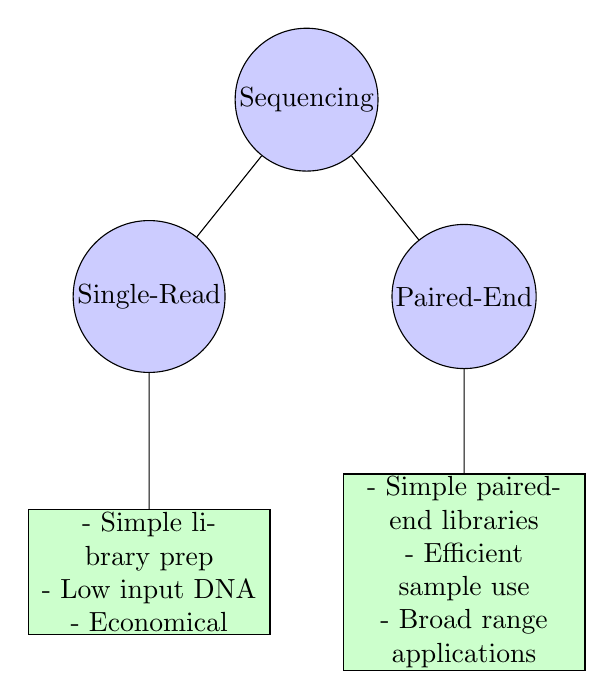
\begin{tikzpicture}[
    every node/.style={draw, circle, fill=blue!20, minimum size=1cm, inner sep=1pt}, % Adjusted minimum size for better text fit
    grandchildnode/.style={draw, rectangle, fill=green!20, text width=3cm, align=center, minimum height=1.5cm}, % Centered text in grandchild
    level 1/.style={sibling distance=4cm, level distance=2.5cm}, % Distance for first level children
    level 2/.style={sibling distance=2cm, level distance=3.5cm}  % Distance for grandchildren
]
\node {Sequencing}
    child {node {Single-Read}
        child {node[grandchildnode] {
            - Simple library prep \\
            - Low input DNA \\
            - Economical
        }} 
    } 
    child {node {Paired-End}
        child {node[grandchildnode] {
            - Simple paired-end libraries \\
            - Efficient sample use \\
            - Broad range applications
        }}
    }; % Semicolon terminates the \node command
\end{tikzpicture}
\end{center}

\textbf{FastA Format:} Most basic for reporting a sequence. Contains sequence name, description. 
\begin{verbatim}
>Chr1 CHROMOSOME dumped from ADB: 
Jun/20/09 14:53; last updated: 2009-02-02
CCCTAAACCCTAAACCCTAAACCCTAAACCTC
TGAATCCTTAATCCCTAAATCCCTAAATCTTT
AAATCCTACATCCAT
\end{verbatim}
\textit{DB query tools} such as \textbf{blast} and \textbf{multiple-sequence alignment} programs accept only FastA. Reference Genomes are often delivered in this format.

\textbf{FastQ Format:} Most widely used in sequence analysis. Output delivered from a sequencer. More information is contained in this format.
\begin{verbatim}
@SEQ_ID
GATTTGGGGTTCAAAGCAGTATCGATCAAATAGTAAATCCAT
TTGTTCAACTCACAGTTT
+
!''*((((***+))%%%++)(%%%%).1***-+*''))**5
5CCF>>>>>>CCCCCCC65
\end{verbatim}
\textit{Quality value characters. Lowest: \texttt{!} and highest: \texttt{\textasciitilde{}}}:
\begin{verbatim}
!"#$%&'()*+,-./0123456789:;<=>?@ABCDEFGHIJKLMN
OPQRSTUVWXYZ[\]^_`abcdefghijklmnopqrstuv
wxyz{|}~
\end{verbatim}

\begin{itemize}
    \item Sequence Header:
    \begin{itemize}
        \item \texttt{@} is sequence identifier
        \item rest is sequence description
    \end{itemize}
    \item Second line is sequence
    \item Third line starts with \texttt{+} and can have same sequence identifier appended
    \item Fourth are quality scores (ASCII encoded)
\end{itemize}
Sequence Header contains: Instrument name, run ID, flowcell ID, flowcell lane, tile number, X and Y coordinates of cluster, member of a pair, filtered status, control bits, index sequence, etc.

Nearly everything works with FastQ except for: Blast, Multiple sequence alignment (typically require FastA), any reference sequence (usually FastA).

\textbf{Quality Scores/Q-score:} Integer value assigned to each nucleotide base. Represents estimated probability ($P$) that base call is incorrect. Logarithmic scale: $Q = -10\log_{10}(P)$.
\textbf{Higher Q-score} = Higher confidence = lower $P$ (error) = higher accuracy.
\textbf{Lower Q-score} = Lower confidence = higher $P$ (error).

\textbf{Examples:}
\begin{itemize}
    \item \textbf{Q10:} $P=0.1$ (1 in 10 error). Accuracy = $90\%$.
    \item \textbf{Q20:} $P=0.01$ (1 in 100 error). Accuracy = $99\%$. Often a minimum acceptable quality.
    \item \textbf{Q30:} $P=0.001$ (1 in 1,000 error). Accuracy = $99.9\%$. Benchmark for high-quality.
    \item \textbf{Q40:} $P=0.0001$ (1 in 10,000 error). Accuracy = $99.99\%$.
\end{itemize}

Common uses: filter bases/reads if a threshold is not met.
Main purpose: provide evidence that the sequence, alignment, assembly, SNP are real and not sequencing artifacts.

\textbf{SAM Format:} Sequence Alignment/Map. Basic, human-readable text format. Generated by most alignment algorithms. Consists of:
\begin{itemize}
    \item \textbf{Header section (optional):} Lines start with \texttt{@}. Contains metadata: SAM format version (\texttt{@HD}), reference sequence dictionary (\texttt{@SQ}), read groups (\texttt{@RG}), program used (\texttt{@PG}), comments (\texttt{@CO})

    \item \textbf{Alignment section:} Each line is an alignment record for a single read. Contains 11 mandatory fields, followed by optional fields. \\

    \textbf{Field Descriptions:}

    \begin{enumerate}
        \item QNAME: Query template NAME
        \item FLAG: bitwise FLAG
        \item RNAME: Reference sequence NAME
        \item POS: 1-based leftmost mapping POSition
        \item MAPQ: MAPping Quality
        \item CIGAR: CIGAR string
        \item RNEXT: Ref. name of the mate/next read
        \item PNEXT: Position of the mate/next read
        \item TLEN: observed Template LENgth
        \item SEQ: segment SEQuence
        \item UAL: ASCII of Phred-scaled base QUALity+33
    \end{enumerate}

\end{itemize}\\

\textbf{BAM:} Same format except that it is encoded in binary(faster to read) but not human legible.\\

\textbf{CRAM:} Retains same info as SAM and is compressed in more efficient way.\\

Formats are \textit{output} from aligners and assemblers 

\textbf{BED Format:} Simple way to define basic sequence features to a sequence. One line per feature, each containing 3 - 12 columns of data plus optional track definition lines. Generally used for user defined sequence features as well as graphical representations of features.

\begin{itemize}
    \item Chromosome Name
    \item Chromosome Start
    \item Chromosome End 
\end{itemize}

\textbf{Optional Fields}
Nine additional fields are optional for feature definition. If higher-numbered optional fields are used, all lower-numbered fields preceding them must also be populated.

\begin{description}
    \item[Name] Label to be displayed under the feature if enabled in the page configuration.
    \item[Score] A numerical score ranging from 0 to 1000. The display style for scored data can be configured using track lines (see below).
    \item[Strand] Defines the orientation of the feature: `+` (forward) or `–` (reverse).
    \item[thickStart] The coordinate where the feature representation begins as a solid rectangle.
    \item[thickEnd] The coordinate where the feature representation as a solid rectangle ends.
    \item[itemRgb] An RGB color value (e.g., 0,0,255). This is applied only if a track line specifies `itemRgb="on"` (case-insensitive).
    \item[blockCount] The number of sub-elements (e.g., exons) within the feature.
    \item[blockSize] A comma-separated list of the sizes of these sub-elements.
    \item[blockStarts] A comma-separated list of the start coordinates for each sub-element, relative to the feature's start coordinate.
\end{description}

\textbf{Track Lines}
Track definition lines configure the display of features, such as grouping them into separate tracks. Track lines must precede the list of features they affect and consist of the word `track` followed by space-separated `key=value` pairs. Valid parameters for Ensembl include:

\begin{description}
    \item[name] A unique identifier for the track when parsing the file.
    \item[description] A label displayed under the track in detailed views (e.g., "Region in Detail").
    \item[priority] An integer determining the display order if multiple tracks are defined.
    \item[color] Specified as RGB, hexadecimal, or an \href{https://www.X.org/releases/X11R7.6/doc/xorg-docs/specs/RGBColorNames.txt}{X11 named color}.
    \item[useScore] A value from 1 to 4, dictating how scored data is displayed. May require additional parameters:
    \begin{itemize}
        \item Tiling array
        \item Colour gradient (defaults to Yellow-Green-Blue with 20 grades). Optionally, custom colors (\texttt{cgColour1}, \texttt{cgColour2}, \texttt{cgColour3}) and the number of grades (\texttt{cgGrades}) can be specified.
        \item Histogram
        \item Wiggle plot
    \end{itemize}
    \item[itemRgb] If set to `on` (case-insensitive), the individual RGB values defined for each feature (in the `itemRgb` field) will be used.
\end{description}

\textbf{BedGraph Format}
The BedGraph format is designed for displaying moderate amounts of scored data and is based on the BED format with these key differences:
\begin{itemize}
    \item The score is located in column 4 (instead of column 5 as in standard BED with score).
    \item Track lines are \textbf{compulsory} and must include `type=bedGraph`.
\end{itemize}
Optional track line parameters currently supported by Ensembl for BedGraph are:
\begin{description}
    \item[name] (as described above)
    \item[description] (as described above)
    \item[priority] (as described above)
    \item[graphType] Specifies the display style, either `bar` or `points`.
\end{description}

\end{literaturepaper}


\begin{literaturepaper}{Latent Variable Models:}
\label{background-info-2}
\small

In convolutional NN lie ResNet-50, there is no semantic understanding of images. Thus models require some form of understanding of uncertainty $\rightarrow$ \textbf{Generative Modeling}.

It aims to model the entire distribution of the input data, including the relationship between the input data and their labels.

Estimation of \textit{Joint Distribution} of input $X$ and labels $Y$.
$P_\theta(X, Y) = P_\theta(Y|X) P_\theta(X)$ can be used to identify outlying data that doesn't belong to any of the trained classes. 
\includegraphics[width = 7cm, height = 3cm]{encode_decode.png}

Another example: \textit{fMRI signals} To generate synthetic data that closely resembles real (medical data sensitivity / privacy issues) for further research.

\textbf{Goal:} To model input and estimate $P(X)$ 

\textbf{Curse of Dimensionality:} As dimensionality of input increases, difficulty in modeling X significantly increases.

\textbf{Pixel Dependency:} Statistical / spatial relationship between value (color/intensity) of one pixel and values of other pixels in an image. 
\begin{itemize}
    \item \textbf{Not independent:} If so, color of 1 pixel would convey 0 information about another pixel.
    \item \textbf{Information Content:} Real-world images contain structure, objects, textures, patterns. They arise because color of 1 pixel is almost always related to the color of its neighboring pixels (and often to pixels further away.
    \item \textbf{Predictability:} Dependencies imply predictability. IF color pixel $+$ dependencies are known, educated guess about color of adjacent pixel.
\end{itemize}

\textbf{Type Pixel Dependencies:}

\begin{itemize}
    \item \textbf{Local Dependencies:}
    \begin{itemize}
        \item \textbf{Spatial Correlation:} PIxels that are physically close to each other tend to have similar values. BLurring Filter average values from local neighborhood. 
       \item \textbf{Edges and Textures:} Sharp change in pixel values over short distance and repeating patterns of pixel values (textures). (in CNN, model learns by looking at small, receptive field (neighborhoods) of pixels. Detection of edges, corners, blobs, based on dependencies within small window).
    \end{itemize}
    \item \textbf{Long-Range/Global Dependencies:} Pixels can also be related across larger distances.
    \begin{itemize}
        \item \textbf{Object Recognition}
        \item \textbf{Contextual Information:} Interpretation OF pixel value can depend on overall context of image. e.g., Path of blue pixels might imply a sky in $X$ image but water in $Y$.
        \item \textbf{Transformers in Vision:} Vvalue of a pixel can be predicted or generated based on the values of previously generated or observed pixels.
    \end{itemize}
\end{itemize}

\textbf{Approaches to modeling dependencies:}

All pixels collectively form a dependence graph, where modeling dependencies is crucial for accurate joint probability estimation $\rightarrow$ highly challenging.

\begin{itemize}
    \item \textbf{Latent Variable Model} defines probability distribution $p(x,z) = p(x|z)p(z)$. \textbf{Sets of variables:} $x =$ Observed variables representing high dimensional observation. $z =$ latent variable not in observation space but hidden and associated with $x$ via $p(z|x)$ and \textbf{\textit{can encode structure of data.}} 

    So idea is to generate hidden factors that generate observed variable $x$. \textbf{Assumption:} $X$ is generated by few independent hidden factors. e.g., \textit{image of face}, latent factors could control gender, eye color, glasses. Assume model $P(X)$ is generated by independent latent factors $Z_1, Z_2,...,Z_n$. Thus latent variable model defines a joint distribution of $P(X)$ and $Z$. (Baye's rule) 
    \end{itemize}
    
    \textit{'how to learn the hidden factors (Z) when only the input (X) is known'}\\

    \textbf{Autoencoder and Compression}

    \begin{itemize}
        \item Linear Encoder: $z = W^Tx$. Linear Decoder: $\hat{x} = Wz$. Minimum error solution $W$ yields same subspace as \textbf{PCA}.
        \begin{itemize}
            \item Project high -dimensional data into low-dimensional space and reconstruct input using low-D structure. $\rightarrow$ Simplify by employing linear mapping
        \end{itemize}
    \end{itemize}

\textbf{Naïve Autoencoder} only learns to reconstruct $X$. (if $z$ has lower dimension than $X$). Latent representation exhibit gaps $\rightarrow$ challenging to infer physical meaning. \\

\includegraphics[width=6cm, height=4cm]{autoencode_lower.png}\\

Separability issues arise where certain regions where images from different digit categories may project into the same space. In \textbf{2D} one may struggle to discern physical meaning of dimensions. e.g., $Z_1$ may encode info about rotation which would be challenging to verify.

\section{Generative Modeling with Latent Variables}\\

\textbf{Generative Process:} \textit{Derivation of Evidence Lower Bound (ELBO) for a latent variable model} (Variational Autoencoders (VAEs)).

\begin{align*}
\ln p_{\theta}(\mathbf{x}) &= \log \int p_{\theta}(\mathbf{x}|\mathbf{z})p_{\lambda}(\mathbf{z})d\mathbf{z} \\
&= \log \int q_{\phi}(\mathbf{z}|\mathbf{x}) \frac{p_{\theta}(\mathbf{x}|\mathbf{z})p_{\lambda}(\mathbf{z})}{q_{\phi}(\mathbf{z}|\mathbf{x})} d\mathbf{z} \\
&\ge \int q_{\phi}(\mathbf{z}|\mathbf{x}) \log \frac{p_{\theta}(\mathbf{x}|\mathbf{z})p_{\lambda}(\mathbf{z})}{q_{\phi}(\mathbf{z}|\mathbf{x})} d\mathbf{z} \quad \\
&= \int q_{\phi}(\mathbf{z}|\mathbf{x}) \left[ \log p_{\theta}(\mathbf{x}|\mathbf{z}) + \log \frac{p_{\lambda}(\mathbf{z})}{q_{\phi}(\mathbf{z}|\mathbf{x})} \right] d\mathbf{z} \\
&= \mathbb{E}_{\mathbf{z} \sim q_{\phi}(\mathbf{z}|\mathbf{x})} [\log p_{\theta}(\mathbf{x}|\mathbf{z})] - D_{KL}(q_{\phi}(\mathbf{z}|\mathbf{x}) || p_{\lambda}(\mathbf{z}))
\end{align*}

\textbf{Goal:} To maximize the marginal log-likelihood of observed data $X$ ($ln(P_\theta)$). $\rightarrow$ Probability of observing $X$ given $\theta$ (model parameters). Model assumes data is generated from latent variables $Z$ through a process $P_\theta(X|Z)$ (\textbf{Decoder}) and $Z$ is drawn from prior distribution $P_\lambda(Z)$ (\textbf{Marginal Prior}).\\

\textbf{Derivation:}

\begin{enumerate}
    \item \textit{Introduction of latent variables:} Marginal likelihood is expressed by integrating out $Z$.

$\ln p_{\theta}(\mathbf{x}) &= \log \int p_{\theta}(\mathbf{x}|\mathbf{z})p_{\lambda}(\mathbf{z})d\mathbf{z}$. 

Where, $P_\theta(X|Z)$ is often modeled by \textit{decoder} and $P_\lambda$ is prior distribution over the latent variables. 

    \item \textit{Introduction \textbf{Variational Posterior (Encoder)}:} Introduction of auxiliary distribution $q_\phi(Z|X)$ to make integral tractable. It aims to approximate posterior $P_\theta(Z|X)$.
    \item \textit{Jensen's Inequality (deriving ELBO):} Since logarithm is concave function, \textbf{Jensen's Inequality ($logE[Y] \geq E[logY]$}, can be applied. Integral can be seen as expectation $E_{q_\theta(Z|X)...}$. THis leads to \textbf{Evidence Lower Bound (ELBO)}.

    Inequality shows that log marginal likelihood $\geq$ ELBO.

$&\ge \int q_{\phi}(\mathbf{z}|\mathbf{x}) \log \frac{p_{\theta}(\mathbf{x}|\mathbf{z})p_{\lambda}(\mathbf{z})}{q_{\phi}(\mathbf{z}|\mathbf{x})} d\mathbf{z} \quad$

   \item \textit{Rewrite ELBO in terms of \textbf{Expectations and KL Divergence}}: 
   
    \textbf{Reconstruction Error/Likelihood:} $Z$ are sampled from the \textit{Variational Posterior ($q_\theta(Z|X)$)}. This encourages \textbf{decoder} to accurately reconstruct $X$ from $Z$ produced by \textbf{encoder} $q_\theta(Z|X)$
    
    $&= \mathbb{E}_{\mathbf{z} \sim q_{\phi}(\mathbf{z}|\mathbf{x})} [\log p_{\theta}(\mathbf{x}|\mathbf{z})]$

    \item \textbf{KL Divergence as Regularization:} Kullback-Leibler divergence between $q_\phi(Z|X)$ and \textit{marginal posterior} $P_\lambda(Z)$. It measures how much 1 probability distribution differs from a 2nd reference probability distribution.
    $D_{KL}(q_{\phi}(\mathbf{z}|\mathbf{x}) || p_{\lambda}(\mathbf{z}))$

    Thus, maximizing ELBO $=$ minimizing KL divergence $\rightarrow$ \textbf{Regularization Term.} encouraging learned $q_\phi(Z|X)$ to be close to the \textbf{prior distribution} over latent variables $Z$ (Often chosen to be a simple distribution).
\end{enumerate}

\includegraphics[width=6cm, height=3cm]{eg_1.png}\\

\includegraphics[width=6cm, height=4.3cm]{eg_2.png}\\

\includegraphics[width=7.3cm, height=1.6cm]{eg_3.png}\\



\end{literaturepaper}


\bibliography{references} % Link to your .bib file

\end{document}